\documentclass[10pt]{beamer}

\usepackage{paratype}
\RequirePackage{cmap}
\RequirePackage[T2A]{fontenc}
\RequirePackage[utf8]{inputenc}

% Set up fonts
%\RequirePackage{paratype} % Arial-like sans serif font
%\RequirePackage{DejaVuSansMono} % Free widespread monospace font with cyrillic support
%\RequirePackage{nimbussans} % Helvetica clone
\RequirePackage[bold,light]{nimbusmono} % Courier clone
%\RequirePackage{tempora}  % "Times" font

\RequirePackage[english,russian]{babel}

\usepackage{amsmath,mathrsfs,amsfonts,amssymb, mathtools}
\usepackage{graphicx, epsfig}
\usepackage{subfig}
\usepackage{setspace}
\usepackage{multirow}
\captionsetup{labelformat=empty}
\usepackage{wrapfig}
\usepackage{array}
\usepackage{multirow}
\usepackage{listings}
\usepackage{color}

\definecolor{dkgreen}{rgb}{0,0.6,0}
\definecolor{gray}{rgb}{0.5,0.5,0.5}
\definecolor{mauve}{rgb}{0.58,0,0.82}

\lstset{frame=tb,
  language=Java,
  aboveskip=3mm,
  belowskip=3mm,
  showstringspaces=false,
  columns=flexible,
  basicstyle={\small\ttfamily},
  numbers=none,
  numberstyle=\tiny\color{gray},
  keywordstyle=\color{blue},
  commentstyle=\color{dkgreen},
  stringstyle=\color{mauve},
  breaklines=true,
  breakatwhitespace=true,
  tabsize=3
}

\usepackage{color, colortbl}
\definecolor{lightRed}{RGB}{240, 170, 150}
\definecolor{lightGreen}{RGB}{170, 230, 150}
\definecolor{lightYellow}{RGB}{240, 230, 180}

\usepackage{changepage}

\setbeamerfont{frametitle}{size=\normalsize,family=\sffamily}
\usetheme{Warsaw}%{Singapore}%{Warsaw}%{Warsaw}%{Darmstadt}
\usecolortheme{sidebartab}
\setbeamertemplate{footline}[author]
\expandafter\def\expandafter\insertshorttitle\expandafter{%
	\insertshorttitle\hfill%
	\insertframenumber\,/\,\inserttotalframenumber}

\definecolor{beamer@blendedblue}{RGB}{3,91,170}
\setbeamercolor{color1}{bg=beamer@blendedblue,fg=white}
% отключить клавиши навигации
\setbeamertemplate{navigation symbols}{}

\usepackage{appendixnumberbeamer}
\usepackage{booktabs}
\usepackage[scale=2]{ccicons}

\usepackage{pgfplots}
\usepgfplotslibrary{dateplot}

\usepackage{xspace}
\newcommand{\themename}{\textbf{\textsc{metropolis}}\xspace}

\usepackage{svg}
\usepackage{todonotes}

\AtBeginSection[]{}

\setbeamertemplate{section in toc}{%
  \alert{$\bullet$}~\inserttocsection}

\graphicspath{{images/}{images2/}{../images/}}

\usepackage{makecell}
\usepackage{changepage}

\title[]{Автоматическая генерация сигнатур сетевых протоколов}
%\subtitle{Подназвание доклада}

\author{Дурнов Алексей Николаевич}

% Russian
\institute[МФТИ]{
    Московский физико-технический институт\\
    Физтех-школа радиотехники и компьютерных технологий\\
    Кафедра системного программирования
    \vspace{0.3cm} \\
    Научный руководитель к.ф-м.н. Гетьман А. И.
}

\date{Москва, 2024 г.}
\titlegraphic{\hfill
\includegraphics[height=0.5cm]{logo_isp_ru.png}}

% English
% \institute{ISP RAS}
% \titlegraphic{\hfill
\includegraphics[height=0.5cm]{logo_isp_en.png}}

\setbeamercolor{footline}{fg=black}

\setbeamerfont{footline}{series=\bfseries}

\begin{document}

\begin{frame}
    \titlepage
    \thispagestyle{empty}
\end{frame}

\begin{frame}{}
    \begin{block}{Методы классификации сетевого трафика:}
        \begin{itemize}
            \item основанные на идентификации по номеру порта сервера
            \item основанные на DPI подходе
            \begin{itemize}
                \item \alert{сигнатурный}
            \end{itemize}
            \item основанные на статистических характеристиках
        \end{itemize}
    \end{block}

    \begin{block}{Сигнатура}
        Это набор байтов (подстрок), обеспечивающий идентификацию.
        Пример сгенерированной сигнатуры для HTTP:
        \begin{itemize}
            \item \{''GET /'', '' HTTP/1.'', ''\textbackslash r\textbackslash nHost: ''\}
        \end{itemize}
    \end{block}

    \begin{block}{Свойства сигнатур для сетевых протоколов}
        \begin{itemize}
            \item короткие общие подстроки
            \item несколько потоков с разным набором подстрок (пример, FTP)
            \item необходимость частого обновления
        \end{itemize}
    \end{block}
\end{frame}

\begin{frame}{Цель и задачи}
    \begin{block}{Цель:}
        разработка и реализация метода автоматической
        генерации сигнатур полезной нагрузки сетевого трафика для его классификации
        в соответствии с использующимся протоколом.
    \end{block}

    \begin{block}{Необходимо решить следующие задачи:}
        \begin{itemize}
            \item провести исследование литературы по соответствующей теме
            \item собрать набор сетевых трасс для последующего тестирования
            \item выбрать формат сигнатуры сетевых протоколов
            \item разработать алгоритм генерации сигнатур
            \item разработать классификатор сетевого трафика для проверки сгенерированных сигнатур
            \item встроить генератор сигнатур и классификатор как модули в систему анализа сетевого трафика, разрабатываемую в ИСП РАН
        \end{itemize}
    \end{block}

\end{frame}

\begin{frame}{Формат сигнатур}
    \begin{itemize}
        \item Сигнатура - набор последовательностей подстрок (байт).
        \item Полезная нагрузка соответствует
        сигнатуре, если она содержит какую-то последовательность подстрок из этого набора.
        \item Иерархия сигнатур:
        \begin{enumerate}
            \item сигнатура содержимого
            \item сигнатура пакета
            \item сигнатура потока
        \end{enumerate}
    \end{itemize}

    \begin{figure}
        \begin{adjustwidth}{-2em}{-2em}
            \centering
            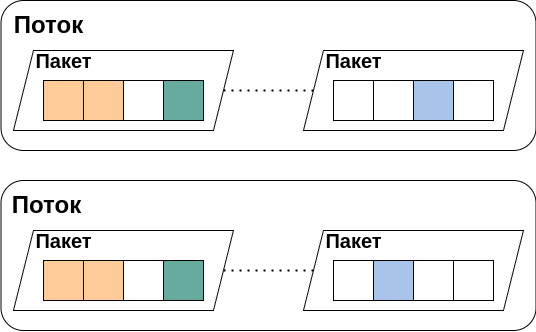
\includegraphics[width=15em]{../images/signature_structure_v2.png}
        \end{adjustwidth}
    \end{figure}

\end{frame}

\begin{frame}{Методы автоматической генерации сигнатур}
    \begin{itemize}
        \item \alert{LASER} (Application Signature ExtRaction)
        \begin{itemize}
            \item \alert{LCS} (Long Common Subsequence)
            \item сигнатура пакета
            \item[+] не требуется сборка сессии
            \item[+] не хранит все потоки
            \item[---] 1 последовательность подстрок
        \end{itemize}
        \item AutoSig
        \begin{itemize}
            \item сигнатура потока
            \item[+] набор последовательностей подстрок
            \item[---] требуется сборка сессии
            \item[---] хранит все потоки
        \end{itemize}
        \item SigBox
        \begin{itemize}
            \item сигнатура потока
            \item[+] не требуется сборка сессии
            \item[---] хранит все потоки
            \item[---] 1 последовательность подстрок
        \end{itemize}
    \end{itemize}

\end{frame}


\begin{frame}{Генерация сигнатур: алгоритм LASER}
    \begin{table}[]
        \resizebox{10cm}{!}{
        \begin{tabular}{|c|c|c|c|}
        \hline
        Протокол  & \begin{tabular}[c]{@{}c@{}} Количество \\ потоков: \\ $\geq$ 5 pkts \end{tabular} & Количество сигнатур & \begin{tabular}[c]{@{}c@{}}Среднее количество \\ потоков на 1 сигнатуру\end{tabular} \\ \hline
        bittorent & 214                                                                               & 51                  & 4,1                                       \\ \hline
        dns       & 11027                                                                             & 682                 & 16,1                                      \\ \hline
        ftp       & 725                                                                               & 9                   & 80,5                                     \\ \hline
        http      & 1500                                                                              & 145                 & 10,3                                      \\ \hline
        imap      & 65                                                                                & 10                  & 6,5                                       \\ \hline
        pop       & 40                                                                                & 2                   & 20,0                                      \\ \hline
        smtp      & 799                                                                               & 167                 & 4,8                                       \\ \hline
        \end{tabular}}
    \end{table}
\end{frame}

\begin{frame}{Результаты работы алгоритма LASER}
    \begin{figure}
        \begin{adjustwidth}{-2em}{-2em}
            \centering
            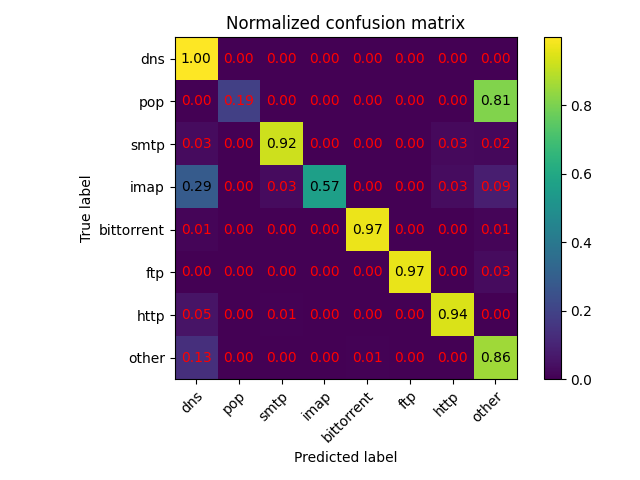
\includegraphics[width=23em]{results/laser_no_filtered/Normalized_confusion_matrix.png}
        \end{adjustwidth}
    \end{figure}
\end{frame}

\begin{frame}{Результаты работы алгоритма LASER}
    \begin{table}[]
        \begin{tabular}{|c|c|c|c|c|}
        \hline
        protocol     & precision & recall & f1-score & support \\ \hline
        dns          & 0.93      & 1.00   & 0.97     & 27801   \\ \hline
        pop          & 0.80      & 0.19   & 0.31     & 21      \\ \hline
        smtp         & 0.94      & 0.92   & 0.93     & 1076    \\ \hline
        imap         & 1.00      & 0.57   & 0.72     & 175     \\ \hline
        bittorrent   & 0.92      & 0.97   & 0.95     & 886     \\ \hline
        ftp          & 0.99      & 0.97   & 0.98     & 295     \\ \hline
        http         & 0.99      & 0.94   & 0.96     & 4888    \\ \hline
        other        & 0.99      & 0.86   & 0.92     & 12094   \\ \hline
                     &           &        &          &         \\ \hline
        accuracy     &           &        & 0.95     & 47236   \\ \hline
        macro avg    & 0.95      & 0.80   & 0.84     & 47236   \\ \hline
        weighted avg & 0.95      & 0.95   & 0.95     & 47236   \\ \hline
        \end{tabular}
        \end{table}
\end{frame}

\begin{frame}{Постобработка: удаление дубликатов и надмножеств}

    \begin{block}{Избыточность}
        Это отношение числа потоков, идентифицированных двумя и более сигнатурами, к общему числу потоков, идентифицированных набором сигнатур.
    \end{block}

    \begin{table}[]
        \resizebox{6cm}{!}{
        \begin{tabular}{|c|cc|cc|}
        \hline
        Протокол & \multicolumn{2}{c|}{\begin{tabular}[c]{@{}c@{}}Количество\\ сигнатур\end{tabular}} & \multicolumn{2}{c|}{Избыточность} \\ \cline{2-5}
                   & \multicolumn{1}{c|}{Было} & Стало & \multicolumn{1}{c|}{Было} & Стало \\ \hline
        bittorrent & \multicolumn{1}{c|}{51}   & 7     & \multicolumn{1}{c|}{0.53} & 0.53  \\ \hline
        dns        & \multicolumn{1}{c|}{682}  & 64    & \multicolumn{1}{c|}{0.99} & 0.99  \\ \hline
        ftp        & \multicolumn{1}{c|}{9}    & 8     & \multicolumn{1}{c|}{0.98} & 0.98  \\ \hline
        http       & \multicolumn{1}{c|}{145}  & 47    & \multicolumn{1}{c|}{1.00} & 1.00  \\ \hline
        imap       & \multicolumn{1}{c|}{10}   & 4     & \multicolumn{1}{c|}{1.00} & 0.79  \\ \hline
        pop        & \multicolumn{1}{c|}{2}    & 1     & \multicolumn{1}{c|}{1.00} & 0.00  \\ \hline
        smtp       & \multicolumn{1}{c|}{167}  & 26    & \multicolumn{1}{c|}{0.99} & 0.99  \\ \hline
        \end{tabular}}
    \end{table}

    \begin{itemize}
        \item Такая постобработка не влияет на результат классификации.
        \item Сильно сократилось количество сигнатур, однако показатель избыточности всё ещё высокий.
    \end{itemize}
\end{frame}


\begin{frame}{Результаты работы алгоритма LASER: \\ со сборкой последовательных пакетов TCP-сессии}
    \begin{figure}
        \begin{adjustwidth}{-2em}{-2em}
            \centering
            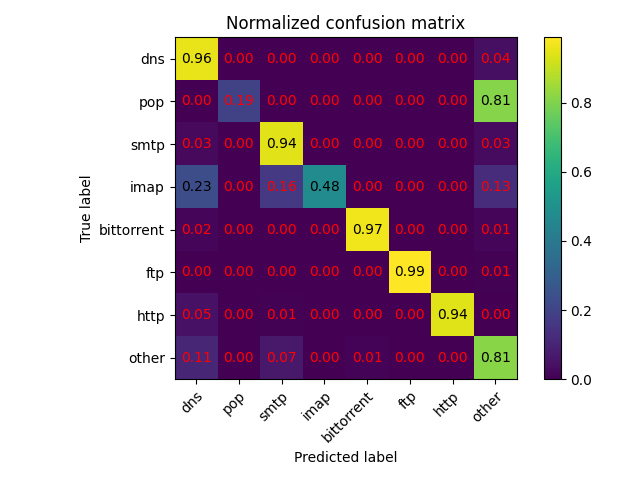
\includegraphics[width=23em]{results/laser_reasm/Normalized_confusion_matrix.png}
        \end{adjustwidth}
    \end{figure}
\end{frame}

\begin{frame}{Результаты работы алгоритма LASER: \\ со сборкой последовательных пакетов TCP-сессии}
    \begin{table}[]
        \resizebox{8cm}{!}{
        \begin{tabular}{|c|c|c|c|c|}
        \hline
        protocol     & precision & recall & f1-score & support \\ \hline
        dns          & 0.92      & 0.96   & 0.94     & 10565   \\ \hline
        pop          & 0.67      & 0.19   & 0.30     &    21   \\ \hline
        smtp         & 0.78      & 0.94   & 0.85     &  1464   \\ \hline
        imap         & 0.91      & 0.48   & 0.62     &   189   \\ \hline
        bittorrent   & 0.95      & 0.97   & 0.96     &   853   \\ \hline
        ftp          & 0.99      & 0.99   & 0.99     &   288   \\ \hline
        http         & 1.00      & 0.94   & 0.97     &  4890   \\ \hline
        other        & 0.88      & 0.81   & 0.85     &  4804   \\ \hline
                     &           &        &          &         \\ \hline
        accuracy     &           &        & 0.92     & 23074   \\ \hline
        macro avg    & 0.89      & 0.79   & 0.81     & 23074   \\ \hline
        weighted avg & 0.92      & 0.92   & 0.92     & 23074   \\ \hline

        \end{tabular}}
    \end{table}

    \begin{itemize}
        \item При частичной сборке TCP-сессии ухудшились несильно.
        \item При полной сборке TCP-сессии, результаты значительно хуже и сильно зависят от ограничения размера рассматриваемой полезной нагрузки.
    \end{itemize}
\end{frame}

\begin{frame}{Схемы генерации сигнатур и классификации трафика}
    \begin{figure}
        \begin{adjustwidth}{-2em}{-2em}
            \centering
            \includesvg[width=27em]{../images/scheme_auto_signature_generation_v2}
        \end{adjustwidth}
    \end{figure}
    \begin{figure}
        \begin{adjustwidth}{-2em}{-2em}
            \centering
            \includesvg[width=31em]{../images/scheme_auto_signature_classifier_v2}
        \end{adjustwidth}
    \end{figure}
\end{frame}


\begin{frame}{Заключение}
    \begin{itemize}
        \item Проведено исследование литературы по соответствующей теме.
        \item Собран набор сетевых трасс для генерации и классификации.
        \item Выбран формат сигнатуры сетевых протоколов.
        \item Рассмотрены ограничения выбранных методов и реализован один из них.
        \item Разработан классификатор сетевого трафика для проверки сгенерированных сигнатур.
        \item Рассмотрено влияние сборки TCP-сессии и постобработки на результат классификации.
        \item Встроены генератор сигнатур и классификатор как модули в систему анализа высокоскоростного сетевого трафика, разрабатываемую в ИСП РАН.
    \end{itemize}
\end{frame}

\begin{frame}{Будущие исследования}
    \begin{itemize}
        \item Реализация и сравнение других методов генерации сигнатур: AutoSig и SigBox.
        \item Реализация модуля уточнения положения сигнатуры и его влияние на точность.
        \item Рассмотрение возможности применения машинного обучения для отбора сигнатур при постобработке результатов.
    \end{itemize}
\end{frame}

\appendix


\begin{frame}[shrink=5]{Данные для генерации сигнатур}
    \begin{table}[]
        \resizebox{12cm}{!}{
            \begin{tabular}{|c|c|c|c|c|c|c|}
                \hline
                Протокол   & \begin{tabular}[c]{@{}c@{}}Размер, \\ МБ\end{tabular} & \begin{tabular}[c]{@{}c@{}}Количество \\ пакетов\end{tabular} & \begin{tabular}[c]{@{}c@{}}Количество \\ потоков\end{tabular} &  \begin{tabular}[c]{@{}c@{}}Avg \\ bytes/pkt \end{tabular} &  \begin{tabular}[c]{@{}c@{}}Avg \\ pkts/stream \end{tabular} & \begin{tabular}[c]{@{}c@{}} Количеcтво \\ потоков: \\ $\geq$ 5 pkts \end{tabular} \\ \hline
                bittorrent & 272,4      & 240159             & 708                & 1134                             & 339                                 & 214                                          \\ \hline
                dns        & 130,7      & 1283082            & 204150             & 102                              & 6                                   & 11027                                        \\ \hline
                ftp        & 0,86       & 16959              & 735                & 51                               & 23                                  & 725                                          \\ \hline
                http       & 1811,5     & 799062             & 13710              & 2268                             & 58                                  & 1500                                         \\ \hline
                imap       & 22,0       & 27702              & 66                 & 793                              & 419                                 & 65                                           \\ \hline
                pop        & 0,06       & 919                & 59                 & 64                               & 16                                  & 40                                           \\ \hline
                smtp       & 13,5       & 59121              & 1120               & 229                              & 53                                  & 799                                          \\ \hline
            \end{tabular}}
    \end{table}
\end{frame}

\begin{frame}[shrink=5]{Данные для классификации}
    \begin{table}[]
        \resizebox{11cm}{!}{
        \begin{tabular}{|c|c|c|c|c|c|}
            \hline
            Протокол   & \begin{tabular}[c]{@{}c@{}}Размер, \\ МБ\end{tabular} & \begin{tabular}[c]{@{}c@{}}Количество \\ пакетов\end{tabular} & \begin{tabular}[c]{@{}c@{}}Количество \\ потоков\end{tabular} &  \begin{tabular}[c]{@{}c@{}}Avg \\ bytes/pkt \end{tabular} &  \begin{tabular}[c]{@{}c@{}}Avg \\ pkts/stream \end{tabular}\\ \hline
            bittorrent & 1,26       & 9409               & 876                & 133                              & 11                                  \\ \hline
            dns        & 53,3       & 664809             & 27800              & 80                               & 24                                  \\ \hline
            ftp        & 0,19       & 4000               & 294                & 48                               & 14                                  \\ \hline
            http       & 1494       & 406030             & 4607               & 3681                             & 88                                  \\ \hline
            imap       & 3,38       & 10587              & 143                & 320                              & 74                                  \\ \hline
            other      & 1119       & 1235122            & 18846              & 906                              & 66                                  \\ \hline
            pop        & 0,02       & 344                & 21                 & 58                               & 16                                  \\ \hline
            smtp       & 5,8        & 34428              & 1018               & 170                              & 34                                  \\ \hline
        \end{tabular}}
    \end{table}
\end{frame}

\begin{frame}{Результаты работы алгоритма LASER: \\ с полной сборкой TCP-сессии}
    \begin{figure}
        \begin{adjustwidth}{-2em}{-2em}
            \centering
            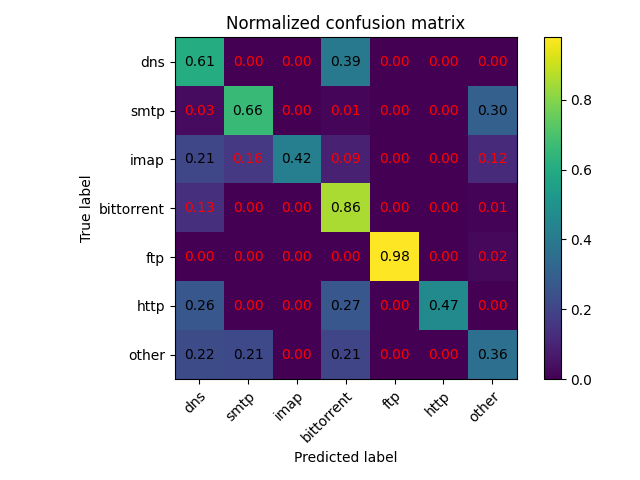
\includegraphics[width=23em]{results/lcs/Normalized_confusion_matrix.png}
        \end{adjustwidth}
    \end{figure}
\end{frame}

\end{document}
